\section{Evaluation der feature-based Algorithmen}
\label{sec:EvaluationFB}

\section{Evaluation SIFT}
\label{sec:EvaluationSIFT}
\begin{figure}[H]
\centering
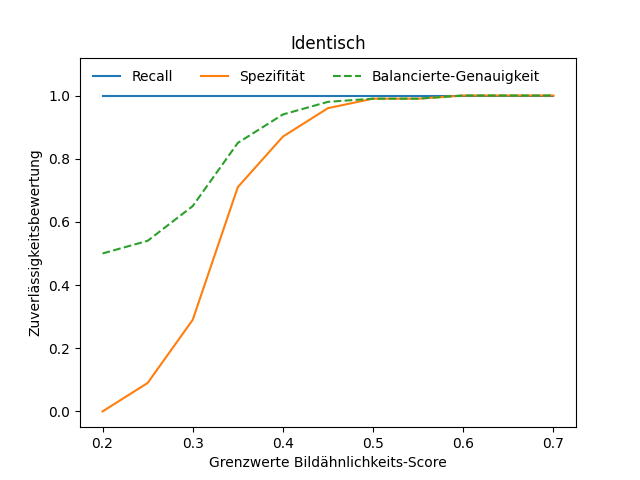
\includegraphics[scale=0.43]{Abbildungen/Evaluation/sift/identical}
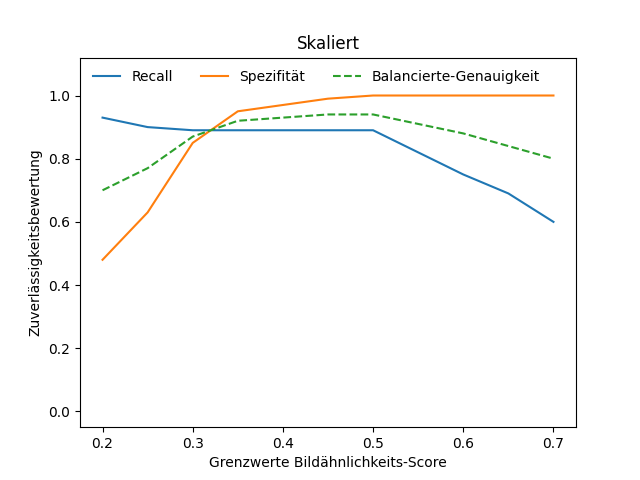
\includegraphics[scale=0.43]{Abbildungen/Evaluation/sift/scaled}
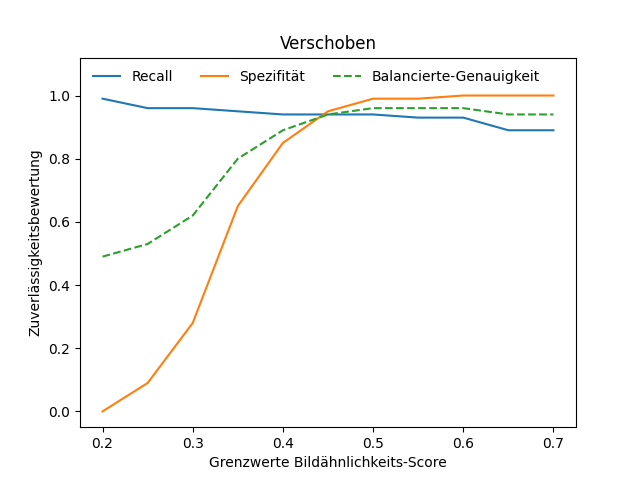
\includegraphics[scale=0.43]{Abbildungen/Evaluation/sift/moved}
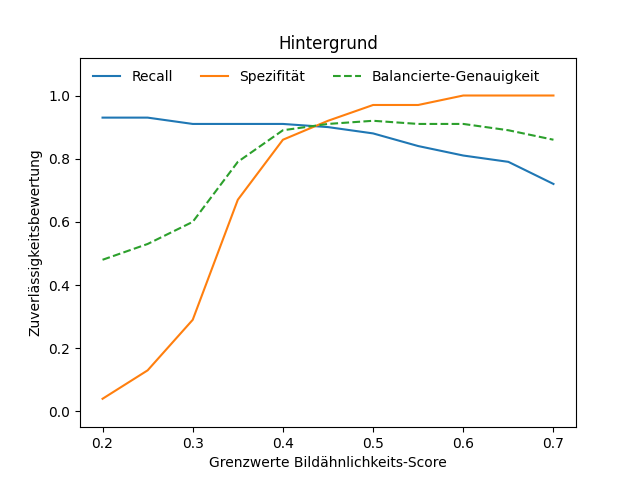
\includegraphics[scale=0.43]{Abbildungen/Evaluation/sift/background}
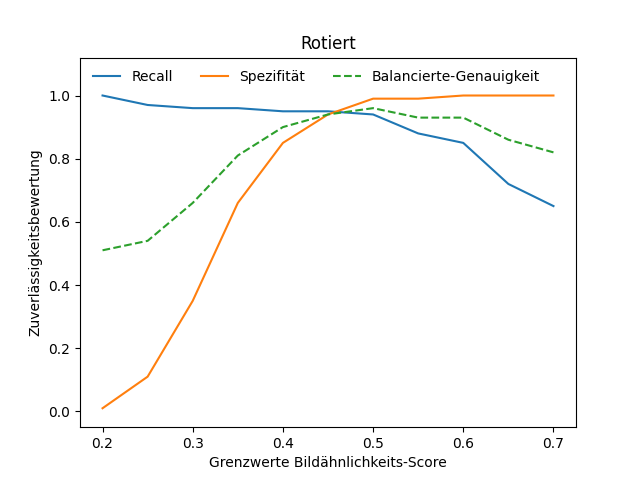
\includegraphics[scale=0.43]{Abbildungen/Evaluation/sift/rotated}
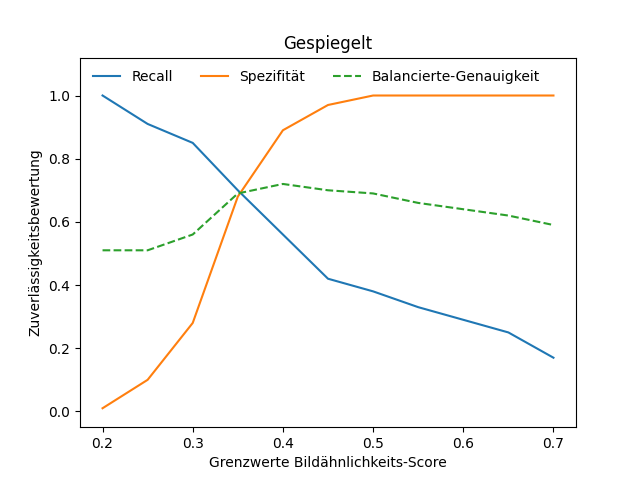
\includegraphics[scale=0.43]{Abbildungen/Evaluation/sift/mirrored}
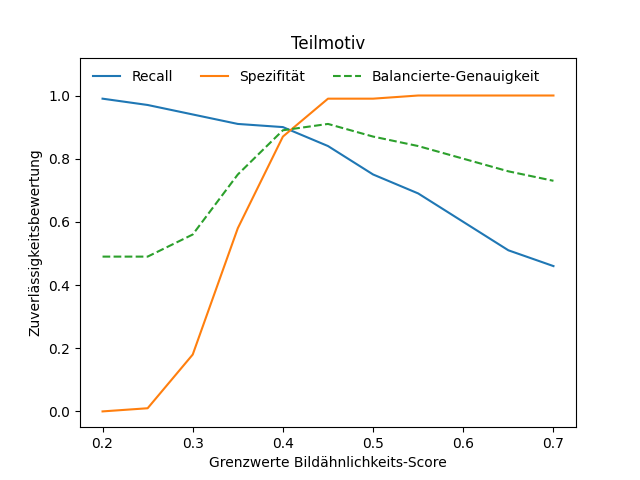
\includegraphics[scale=0.43]{Abbildungen/Evaluation/sift/part}
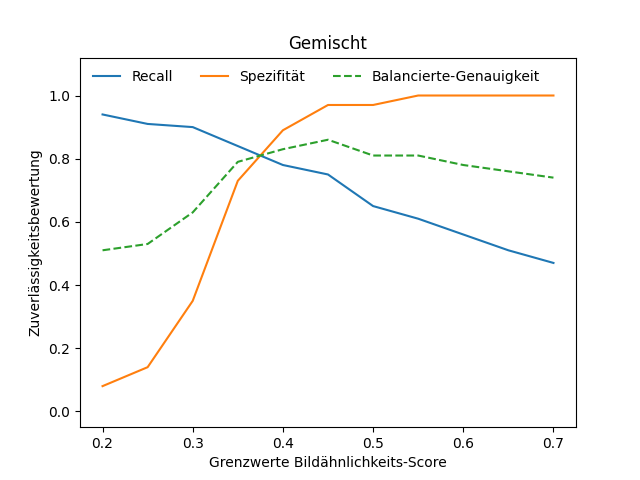
\includegraphics[scale=0.43]{Abbildungen/Evaluation/sift/mixed}
\caption{Zuverl�ssigkeit des SIFT Algorithmus in mehreren Szenarien �ber mehrere Grenzwerte f�r den Bild�hnlichkeits-Score}
\label{fig:phash-standard}
\end{figure}

\section{Evaluation ORB}
\label{sec:EvaluationORB}
\begin{figure}[H]
\centering
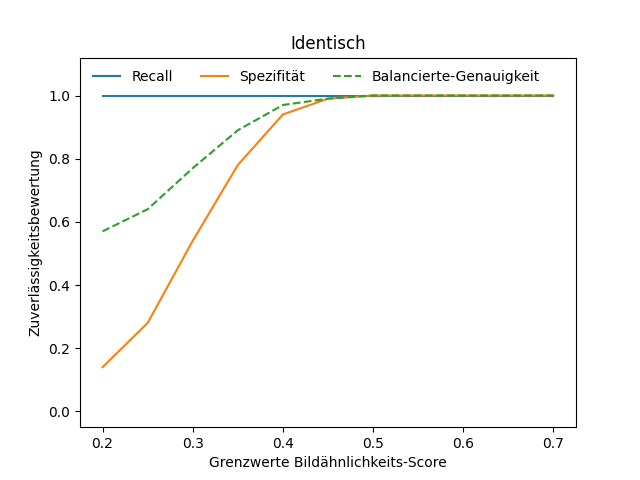
\includegraphics[scale=0.43]{Abbildungen/Evaluation/orb/identical}
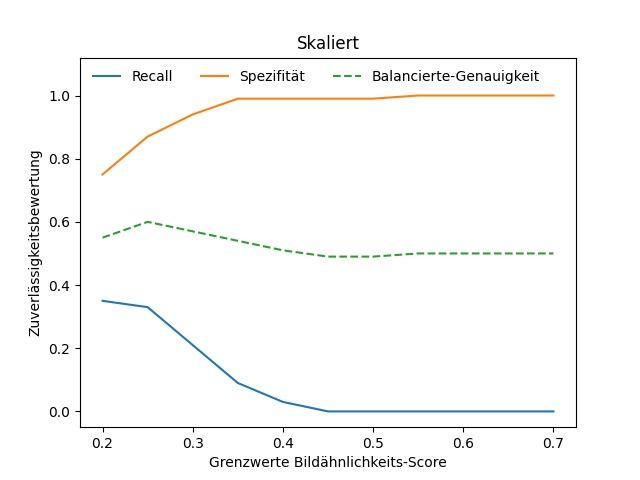
\includegraphics[scale=0.43]{Abbildungen/Evaluation/orb/scaled}
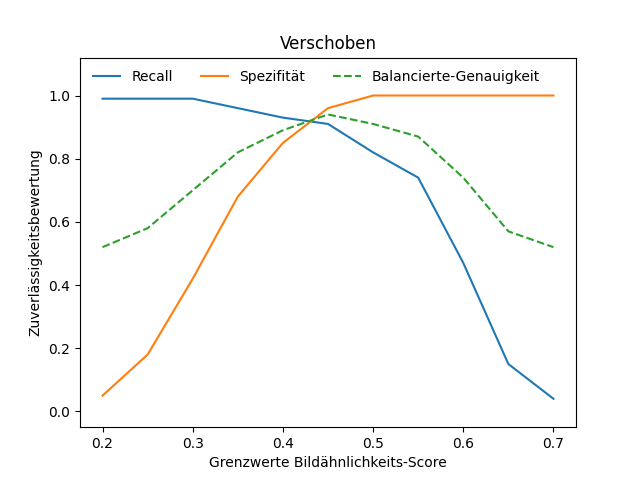
\includegraphics[scale=0.43]{Abbildungen/Evaluation/orb/moved}
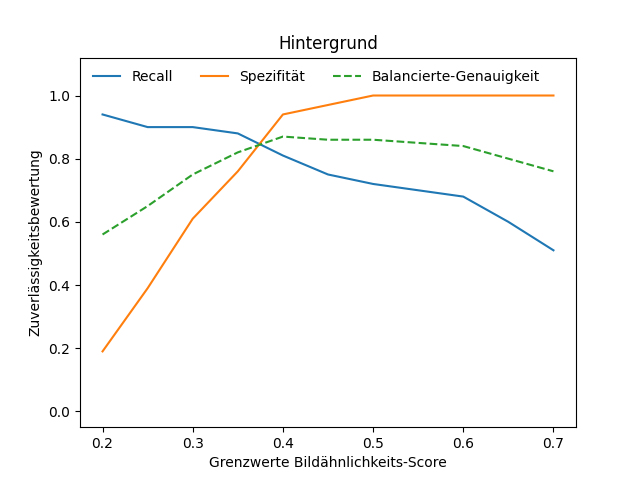
\includegraphics[scale=0.43]{Abbildungen/Evaluation/orb/background}
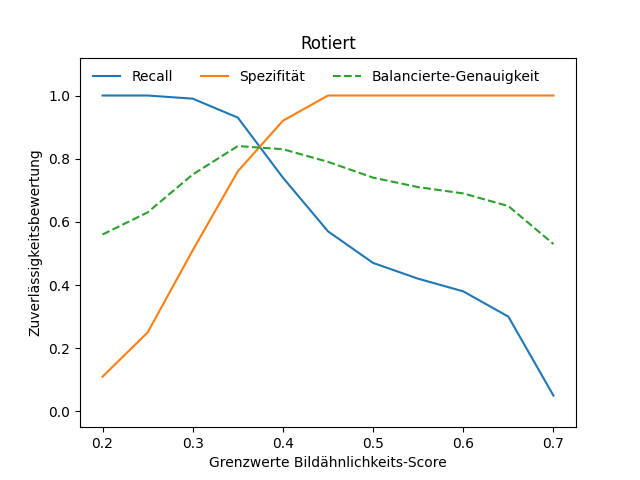
\includegraphics[scale=0.43]{Abbildungen/Evaluation/orb/rotated}
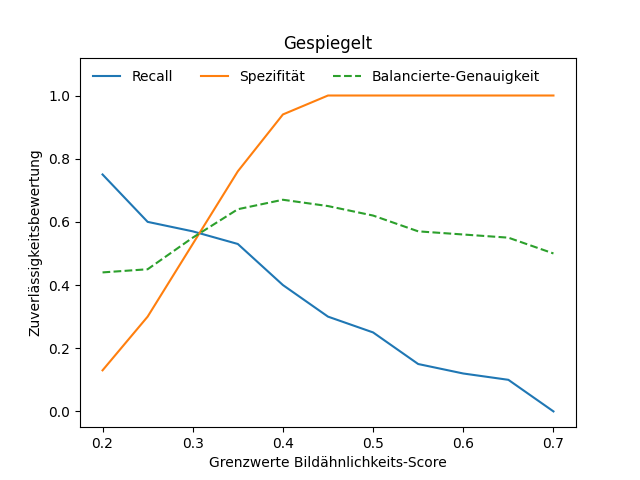
\includegraphics[scale=0.43]{Abbildungen/Evaluation/orb/mirrored}
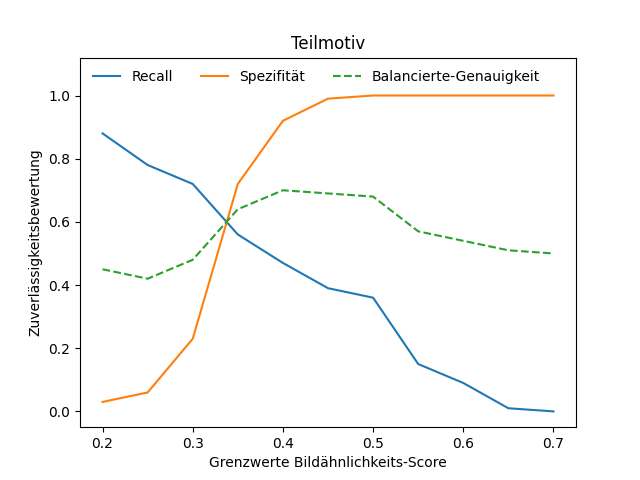
\includegraphics[scale=0.43]{Abbildungen/Evaluation/orb/part}
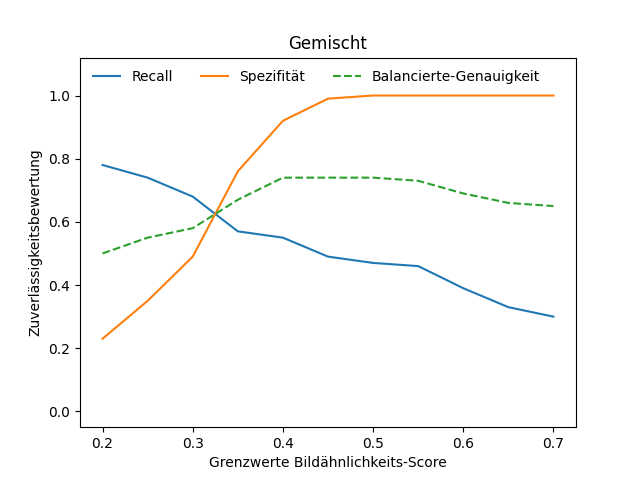
\includegraphics[scale=0.43]{Abbildungen/Evaluation/orb/mixed}
\caption{Zuverl�ssigkeit des ORB Algorithmus in mehreren Szenarien �ber mehrere Grenzwerte f�r den Bild�hnlichkeits-Score}
\label{fig:phash-standard}
\end{figure}

\section{Evaluation BRISK}
\label{sec:EvaluationBRISK}
\begin{figure}[H]
\centering
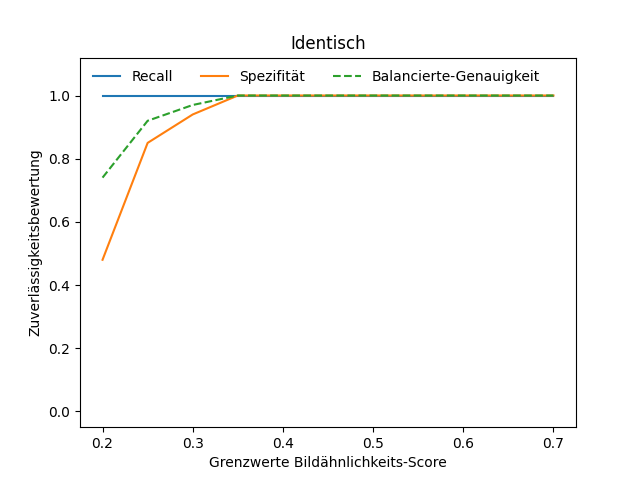
\includegraphics[scale=0.43]{Abbildungen/Evaluation/brisk/identical}
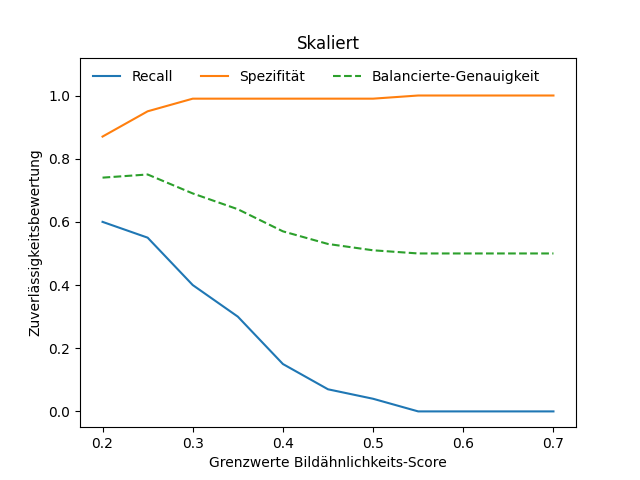
\includegraphics[scale=0.43]{Abbildungen/Evaluation/brisk/scaled}
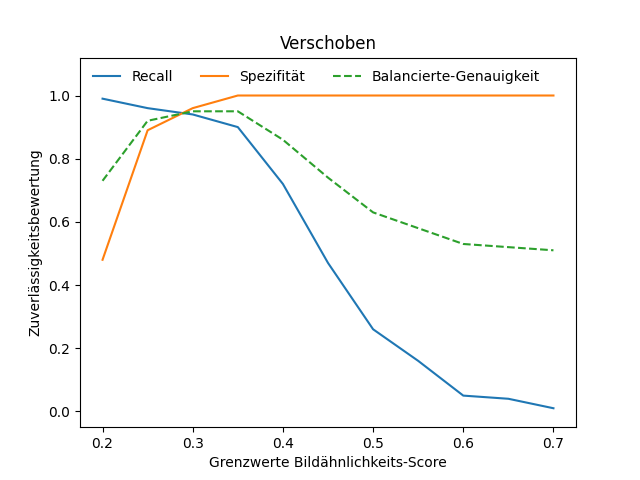
\includegraphics[scale=0.43]{Abbildungen/Evaluation/brisk/moved}
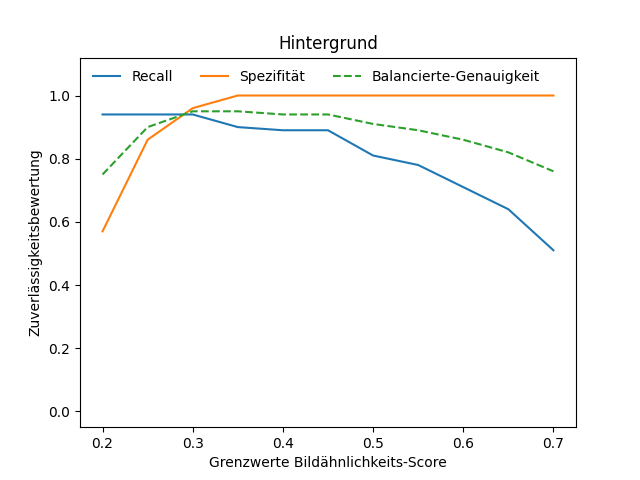
\includegraphics[scale=0.43]{Abbildungen/Evaluation/brisk/background}
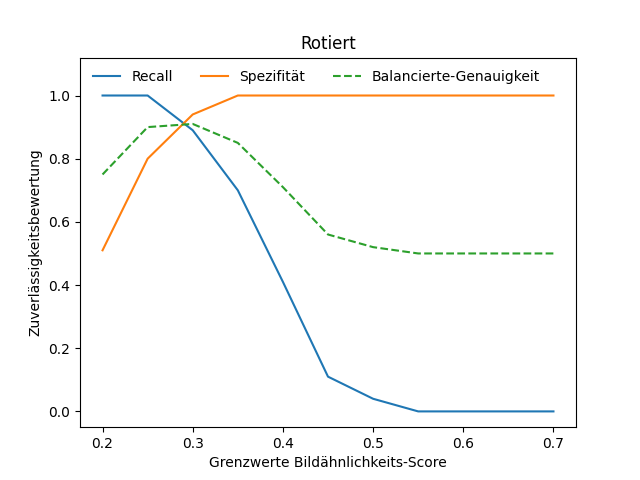
\includegraphics[scale=0.43]{Abbildungen/Evaluation/brisk/rotated}
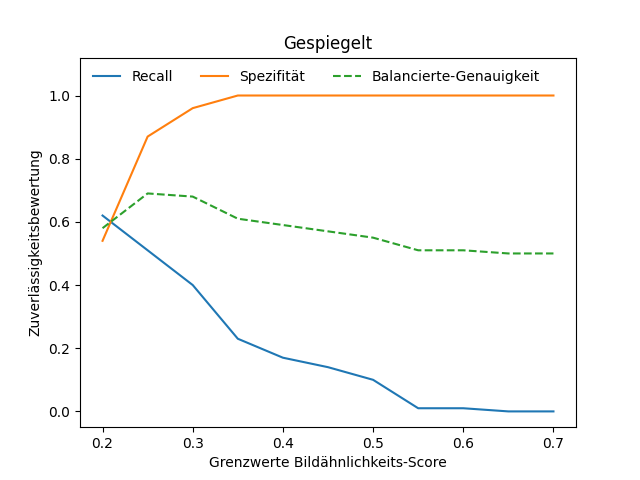
\includegraphics[scale=0.43]{Abbildungen/Evaluation/brisk/mirrored}
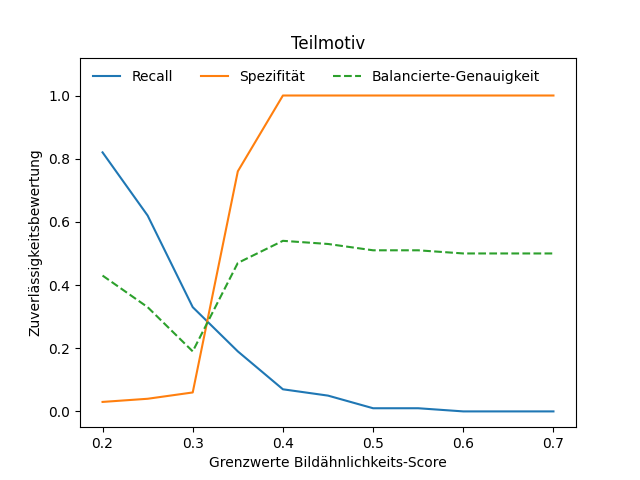
\includegraphics[scale=0.43]{Abbildungen/Evaluation/brisk/part}
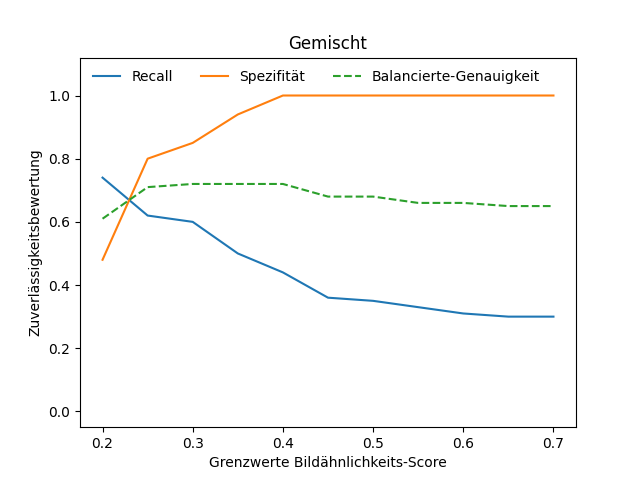
\includegraphics[scale=0.43]{Abbildungen/Evaluation/brisk/mixed}
\caption{Zuverl�ssigkeit des BRISK Algorithmus in mehreren Szenarien �ber mehrere Grenzwerte f�r den Bild�hnlichkeits-Score}
\label{fig:phash-standard}
\end{figure}